% $Header: /cvsroot/latex-beamer/latex-beamer/solutions/generic-talks/generic-ornate-15min-45min.en.tex,v 1.5 2007/01/28 20:48:23 tantau Exp $

\documentclass{beamer}
%\documentclass[handout]{beamer}
%\usepackage{pgfpages}
%\pgfpagesuselayout{2 on 1}[a4paper,border shrink=5mm]

\newcommand{\Href}[1]{\htmladdnormallink{#1}{#1}}
\newcommand\Qt{\"{}}                   % Double quotes...
\newcommand\Bs{\char '134}             % Backslash character for the \tt font
\newcommand\Or{\texttt{|}\,\,}         % Logical Or
\newcommand\BPipe{\,\rule[-.8ex]{1.8pt}{2.6ex}\,}
\newcommand\BOr{\BPipe}    % Logical Or (bold)
\newcommand\Nl{'{\Bs}0'}               % Nul character in C ('\0')
\newcommand\rarrow{$\longrightarrow$ } % A rightarrow


% This file is a solution template for:

\mode<presentation>
{
  \usetheme{Fdc}
  % or ...

  %\setbeamercovered{transparent}
  \setbeamercovered{invisible}
  % or whatever (possibly just delete it)
}


\usepackage[english]{babel}

\usepackage[latin1]{inputenc}

\usepackage{times}
\usepackage[T1]{fontenc}


\title[Wavelet-Based Image Search] % (optional, use only with long paper titles)
{A Wavelet-Based, Image-Property-Based Image Search Engine}


\author{Martin~Dietze}

\institute{Freiheit.com Technologies}

\date[Short Occasion] % (optional)
{May 14, 2009 / Hacker Talk}

\subject{Talks}
% This is only inserted into the PDF information catalog. Can be left
% out. 


\def\RImageSize{0.2\textwidth}
\def\RImageSpace{\hspace{1cm}}


\begin{document}

\begin{frame}
  \titlepage
\end{frame}

\begin{frame}{Outline}
  \tableofcontents
  % You might wish to add the option [pausesections]
\end{frame}


\section{Introduction}
\subsection{Introduction}

\begin{frame}
  \frametitle{Introduction}

  \begin{block}{Goals}<1->
    \begin{itemize}
    \item Image query by perceptual features / similarity
    \item Matches ``as good as possible''
    \item Query against scanned or hand-drawn images
    \end{itemize}
  \end{block}

  \begin{block}{Technically}<2->
    \begin{itemize}
    \item Fast, modest memory footprint, web interface
    \item Idea: Fast Multiresolution Image Querying \emph{[Jacobs95]}
    \item Wavelet-based approach
    \end{itemize}
  \end{block}
\end{frame}

\subsection{Background}

\subsection{Wavelets}

\begin{frame}
  \frametitle{Wavelets}

  \begin{block}{Basics}<1->
    \begin{itemize}
    \item ``Small Waves'' applied on data in different scales
    \item Change of basis
    \item Combined space / frequency domain representation
    \end{itemize}
  \end{block}

  \begin{block}{Base Functions}<2->
    \begin{itemize}
    \item \emph{Wavelet Function}: $\psi_\lambda (x)$ with $\psi$ from a function
      space $\cal F$,\\
      $x$ from a spatial domain $X$ and $\lambda$ from an index domain $\Lambda$.
    \item And, accordingly, \emph{Scaling Function}:  $\phi_\lambda (x)$  
    \end{itemize}
  \end{block}
\end{frame}

\begin{frame}
  \frametitle{Examples}

  \begin{figure}[hbt]
    \begin{center}
      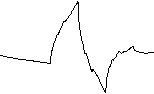
\includegraphics[width=\RImageSize]{daubechies-d4-wavelet.jpg}
      \RImageSpace
      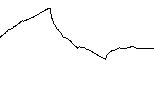
\includegraphics[width=\RImageSize]{daubechies-d4-scaling.jpg}
      \caption{The Daubechies D4 Wavelet and Scaling Functions}
    \end{center}
  \end{figure}

  \pause
  \begin{figure}[hbt]
    \begin{center}
      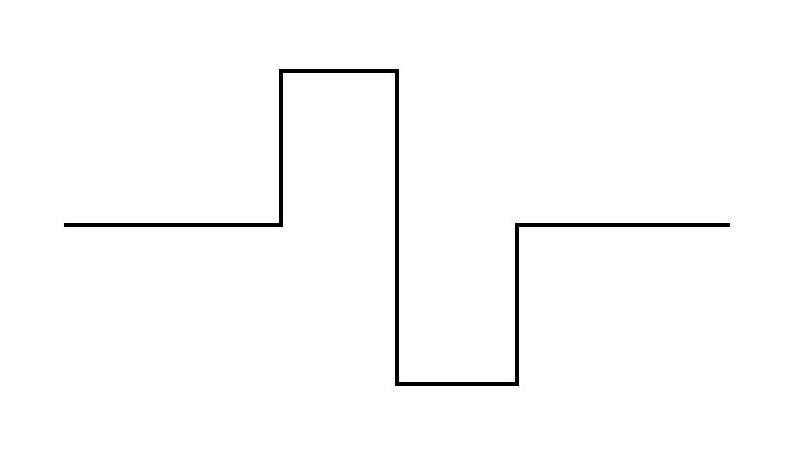
\includegraphics[width=\RImageSize]{haar-wavelet.jpg}
      \RImageSpace
      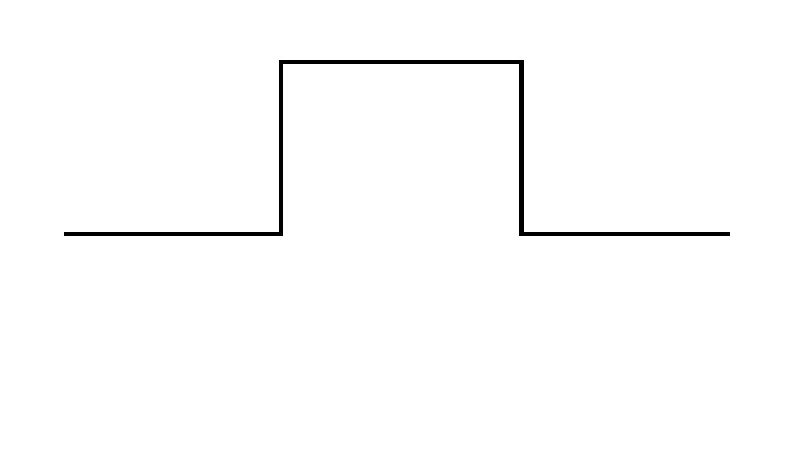
\includegraphics[width=\RImageSize]{haar-scaling.jpg}
      \caption{The Haar Wavelet and Scaling Functions}
    \end{center}
  \end{figure}

\end{frame}

\begin{frame}
  \frametitle{Decomposition}

  \begin{figure}[hbt]
    \begin{center}
      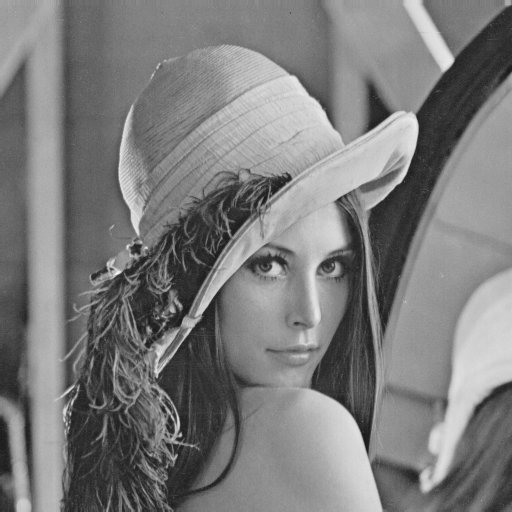
\includegraphics[width=\RImageSize]{lena512.jpg}
      \RImageSpace
      \pause
      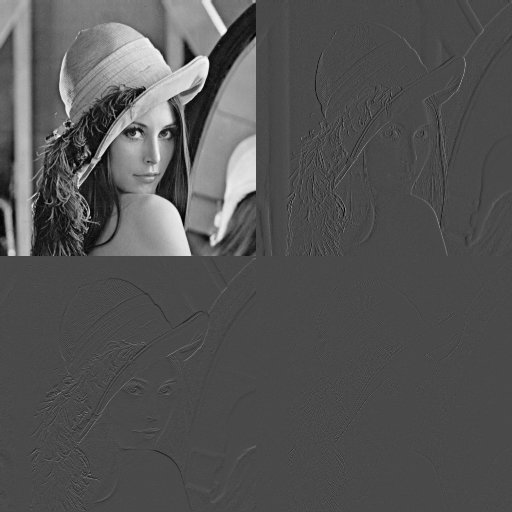
\includegraphics[width=\RImageSize]{lena-1step.jpg}
    \end{center}
  \end{figure}
  \pause
  \begin{figure}[hbt]
    \begin{center}
      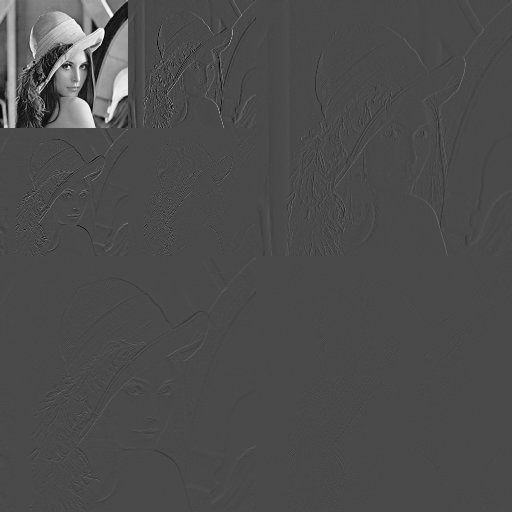
\includegraphics[width=\RImageSize]{lena-2step.jpg}
      \RImageSpace
      \pause
      
\includegraphics[width=\RImageSize]{lena-9step.jpg}
      \caption{Decomposing Lena}
    \end{center}
  \end{figure}

\end{frame}

\section{Application}
\subsection{Algorithm}

\begin{frame}
  \frametitle{Algorithm}

  \begin{block}{Score Table}<1->
    \begin{itemize}
    \item \emph{YUV} colour space, normalised size, mirror extension
    \item Perform a full \emph{Haar} Decomposition on the image
    \item Keep the most significant $k$ (parameter) values as $\pm 1$
    \end{itemize}
  \end{block}

  \begin{block}{Preprocessing}<2->
    \begin{itemize}
    \item \emph{plus} and \emph{minus} table per colour channel $c$:
      $T_{c,\{+|-\}}$
    \item $YX$ ($Y$ rows, $X$ cols) binary arrays $A_{c,\{+|-\},y,x}$ per table
    \item Image $I_n$: $A_{c,\{+|-\},y,x,n} :=
      \mbox{significant}(I_{n,y,x}) \,\&\&\, \mbox{signs match}$
    \end{itemize}
  \end{block}

\end{frame}

\begin{frame}
  \frametitle{Algorithm}

  \begin{block}{Score Initialisation}<1->
    \begin{itemize}
    \item Same transform and quantisation as for the score table
    \item Initial score $L_q$ (query image $Q$, database image $I_n$):

      \medskip
      ~~$L_{q,n} := \sum_{c} \mbox{abs}(Q_{c,0,0} - I_{n,c,0,0})$
    \end{itemize}
  \end{block}

  \begin{block}{Score on Detail Coefficients}<2->
    \begin{itemize}
    \item For each Image $I_n$, position $(y,x)$, colour
      channel $c$:\vspace{4pt}
      \begin{itemize}
      \item Array:~~ $A_{n,c,y,x} := Q_{c,y,x} > 0 \mbox{~?~} A_{n,c,+,y,x}
        \mbox{~:~} A_{n,c,-,y,x}$\vspace{4pt}
      \item If ~$A_{n,c,y,x}$ ~matches: ~~$L_{q,n} -= \mbox{weight(y,x)}$\vspace{4pt}
      \end{itemize}
    \end{itemize}
  \end{block}

  \pause
  \rarrow The lower the score value the better the match
\end{frame}

\subsection{Implementation}

\begin{frame}
  \frametitle{Implementation}

  \begin{block}{Technically}<1->
    \begin{itemize}
    \item C++, libstdc++, some boost libraries \emph{[boost]}
    \item My own Wavelet library \emph{[libWavelet]}
    \item PostgresQL and a C++ API \emph{[pqxx]}
    \item WT Web Toolkit \emph{[wt]}
      \pause
    \item And: \texttt{M-x viper-mode} :)
    \end{itemize}
  \end{block}

  \begin{block}{Initial Approach}<3->
    \begin{itemize}
    \item Image IDs bitwise as offsets in \emph{plus} and \emph{minus} arrays
    \end{itemize}
  \end{block}
\end{frame}

\begin{frame}
  \frametitle{Implementation}

  \begin{block}{Optimisation}<1->
    \begin{itemize}
    \item Quest for better runtime performance
    \item Initial assumption: faster queries, bigger memory footprint
    \item Alternative Score Table \rarrow \emph{OPEN IMPLEMENTATION}\\
      \texttt{ScoreTableFactory::create (/*...*/, SPEED)}\\
      \texttt{ScoreTableFactory::create (/*...*/, SIZE)}\\
    \end{itemize}
  \end{block}

  \begin{block}{Second Approach}<2->
    \begin{itemize}
    \item Keep matching images' IDs in \emph{plus} and \emph{minus} arrays
    \end{itemize}
  \end{block}

  \pause
  \rarrow More work at setup, fewer comparisons when querying
\end{frame}

\section{Results and Discussion}

\subsection{Results}

\begin{frame}
  \frametitle{Comparison of the Approaches}

    \begin{block}{Experimental Results (610 images, 60 kept coefficients)}
      \begin{center}
        \begin{tabular}{|l|r|r|}\hline
          ~ & \texttt{SIZE} & \texttt{SPEED} \\ \hline\hline
          Initial Setup Time & 13.2 sec & 8.2 sec \\ \hline
          Average Query Time & 4.0 ms  & 0.0 ms \\ \hline
          Score Table Size & 29.98 MB  & 6.29 MB \\ \hline
        \end{tabular}
      \end{center}
    \end{block}

    \pause
    \begin{itemize}
      \item The \texttt{SPEED} variant takes \emph{less} space

        \pause
        \rarrow \texttt{\%s/SIZE/BAD/g}\pause, \texttt{\%s/SPEED/GOOD/g} \pause :)
      \end{itemize}

\end{frame}

\begin{frame}
  \frametitle{Technology Impressions \#1}

  \begin{block}{Wavelet-Lib}<1->
    \begin{itemize}
    \item 26,000 lines of C++ code
    \item Rather old (started in 1999)
    \item No STL, no smart pointers, prone to memory leaks
    \item Nevertheless well-tested (thanks to \emph{valgrind})
    \end{itemize}
  \end{block}

  \begin{block}{Pqxx}<2->
    \begin{itemize}
    \item Poor documentation, tedious to use, PostgresQL only
    \item Better try \emph{hiberlite} or \emph{sqlite} in future!
    \end{itemize}
  \end{block}
  
\end{frame}

\begin{frame}
  \frametitle{Technology Impressions \#2}

  \begin{block}{WT}<1->
    \begin{itemize}
    \item Elegant, QT-like API (\rarrow \emph{Signals}, \emph{Slots})
    \item Good CSS and Ajax integration
    \item Very code-based, HTML templates difficult to integrate
    \item After little time, productivity felt quite good, a bit like
      \emph{Wicket}
    \end{itemize}
  \end{block}
  \begin{block}{Technology which was \emph{not} used}<2->
    \begin{itemize}
    \item \emph{Spring}; handwritten wiring of services was
      still simple enough, but with increasing size...
    \end{itemize}
  \end{block}
  
\end{frame}

\subsection{Summary}

\begin{frame}{Summary}

  \begin{block}{Results}<1->
    \begin{itemize}
    \item The image search engine is fast and memory efficient
    \item Results are good on images with few details
    \item Images of landscapes are problematic
    \end{itemize}
  \end{block}
  
  \begin{block}{Future Work}<2->
    \begin{itemize}
    \item Rewrite the database backend code and get rid of \emph{pqxx}
    \item More experiments with different weight factors and
      numbers-of-kept-coefficients
    \end{itemize}
  \end{block}
  
  \begin{itemize}
  \item<3-> That's all, folks!
  \end{itemize}

\end{frame}

\subsection{References}

\begin{frame}{References}

  \begin{description}
  \item[\textit{[Jacobs95]}] Charles E. Jacobs and Adam Finkelstein and David H. Salesin, \emph{Fast Multiresolution Image Querying}, Computer Graphics \#29, 1995
  \item[\textit{[libWavelet]}] Martin Dietze, \emph{Wavelet library}, \Href{http://herbert.the-little-red-haired-girl.org/en/wavelet/index.html}

  \item[\textit{[boost]}] Various, \emph{Boost libraries}, \Href{http://www.boost.org}

  \item[\textit{[pqxx]}] Various, \emph{Pqxx PostgresQL wrapper}, \Href{http://pqxx.org}

  \item[\textit{[wt]}] Various, \emph{WT Web Toolkit}, \Href{http://www.webtoolkit.eu}
  \end{description}

\end{frame}

\end{document}


